%!TEX root = main.tex


\frontmatter % Use roman page numbering style (i, ii, iii, iv...) for the pre-content pages

\pagestyle{plain} % Default to the plain heading style until the thesis style is called for the body content

%----------------------------------------------------------------------------------------
%	TITLE PAGE
%----------------------------------------------------------------------------------------

\begin{titlepage}
\begin{center}

\vspace*{.02\textheight}
%{\scshape\LARGE \univname\par}\vspace{1.5cm} % University name
% \bigskip  
%\textsc{\Large Doctoral Thesis}\\[0.5cm] % Thesis type

%\HRule \\[0.4cm] % Horizontal line

%{\huge \bfseries \ttitle\par}\vspace{0.6cm} % Thesis title automatic

{\bfseries
\LARGE{Decision theoretic foundations for\\ statistical causal modelling}\\
\bigskip
\large{}
}

\vspace{1cm} % Thesis title

%\HRule \\[1.2cm] % Horizontal line
 
\begin{minipage}[t]{0.3\textwidth}
\begin{center}
 \large
%\emph{Author:}\\
 \authorname % Author name - remove the \href bracket to remove the link
\end{center}
\end{minipage}

%\begin{minipage}[t]{0.4\textwidth}
%\begin{flushright} \large
%\emph{Supervisor:} \\
%\href{http://www.jamessmith.com}{\supname} % Supervisor name - remove the \href bracket to remove the link  
%\end{flushright}
%\end{minipage}\\[3cm]
 
% \vspace{1cm}
% 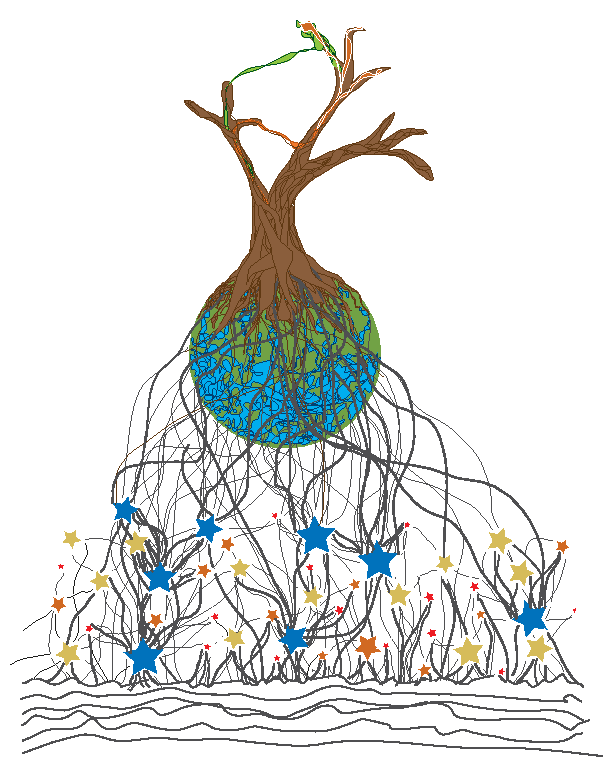
\includegraphics[width=0.6\textwidth]{gfx/front_cover} \\ \bigskip  
% \vspace{1cm}

\large \textit{A thesis submitted for the degree of \degreename}\\[0.7cm] % University requirement text
%\textit{in the}\\[0.4cm]
% \groupname\\
\deptname\\ % Research group name and department name
%\univname % University name

%{\small Draft (\today)}\\[2cm] % Date
%\includegraphics{Logo} % University/department logo - uncomment to place it


\includegraphics[width=5cm]{gfx/ANU_LOGO_cmyk_56mm}

{\normalsize September, 2022}\\[2cm] % Date
\vspace*{\fill}

\copyright Copyright by \authorname  2022

All Rights Reserved
\end{center}

\end{titlepage}

%----------------------------------------------------------------------------------------
%	DECLARATION PAGE
%----------------------------------------------------------------------------------------

\begin{declaration}
%\addchaptertocentry{\authorshipname} % Add the declaration to the table of contents
\begingroup
\large
\noindent This thesis is an account of research undertaken between January 2018 and September 2022 at the College of Engineering and Computer Sciences, The Australian National University, Canberra, Australia. 

%Except where acknowledged in the customary manner, all material presented in this dissertation including figures and photographs are original and have not been submitted in whole or part for a degree in any university.

The work presented in this thesis is that of the candidate alone, except where indicated by due literature reference and acknowledgements in the text. It has not been submitted in whole or in part for any other degree at this or any other university.

The development of ideas and research was undertaken with guidance from my primary supervisors Robert Williamson and Cheng Soon Ong, and the thesis was written by myself. The overall direction of the research was developed in collaboration with my supervisors, who also provided a lot of detailed feedback on my work along the way. The original results presented here were primarily my work.

\bigskip
\vspace{1cm}
\begin{flushright}
\authorname\\
\today
\end{flushright}
\endgroup
\end{declaration}
\vspace{3cm}
% \begingroup
% \footnotesize\emph{{Cover: Figure 1 from \fullcite{Lineweaver2012AnnRev}}}
% \endgroup
\cleardoublepage

% \begin{declaration}
% \addchaptertocentry{\authorshipname} % Add the declaration to the table of contents
% \noindent I, \authorname, declare that this thesis titled, \enquote{\ttitle} and the work presented in it are my own. I confirm that:

% \begin{itemize} 
% \item This work was done wholly or mainly while in candidature for a research degree at this University.
% \item Where any part of this thesis has previously been submitted for a degree or any other qualification at this University or any other institution, this has been clearly stated.
% \item Where I have consulted the published work of others, this is always clearly attributed.
% \item Where I have quoted from the work of others, the source is always given. With the exception of such quotations, this thesis is entirely my own work.
% \item I have acknowledged all main sources of help.
% \item Where the thesis is based on work done by myself jointly with others, I have made clear exactly what was done by others and what I have contributed myself.\\
% \end{itemize}
 
% \noindent Signed:\\
% \rule[0.5em]{25em}{0.5pt} % This prints a line for the signature
 
% \noindent Date:\\
% \rule[0.5em]{25em}{0.5pt} % This prints a line to write the date
% \end{declaration}

% \cleardoublepage

%----------------------------------------------------------------------------------------
%	QUOTATION PAGE
%----------------------------------------------------------------------------------------

% \vspace*{0.2\textheight}

% \noindent\enquote{\itshape Thanks to my solid academic training, today I can write hundreds of words on virtually any topic without possessing a shred of information, which is how I got a good job in journalism.}

% \hfill Dave Barry

%----------------------------------------------------------------------------------------
%	ACKNOWLEDGEMENTS
%----------------------------------------------------------------------------------------

\begin{acknowledgements}
\addchaptertocentry{\acknowledgementname} % Add the acknowledgements to the table of contents
\vspace{0.4cm}
\begingroup
\normalsize
The research in this thesis would not have been possible without my primary supervisors Robert Williamson, Cheng Soon Ong and Amanda Barnard. They have all been extremely patient, they have provided enormous amounts of good advice and discussion about technical details of my research, writing and about where I might be trying to go in the end and how I might get there. This research was motivated by a seemingly compelling idea about the relationship between causal models and the purpose of causal modelling, and a great deal of time was taken up with struggling to fashion this idea into a coherent and comprehensible theory. I sometimes doubted whether there was a worthwhile payoff in the end, or whether I would be able to find it. The support from my supervisors in all its forms helped me to find a path forward and to believe it was still a path worth following.

I would also like to thank Parastoo Sadeghi, Tom Everitt, Sarita Rosenstock and Zhen-Yue Chin for listening to my ideas, offering feedback, encouragement and organisational advice, and Amardeep Wander for offering flexible employment throughout much of the time I have been working on this research. Both the flexibility and the employment are deeply appreciated. I would also like to thank my parents Julie Permezel and Dennis Johnston for their help with childcare at the end of writing.

I would finally like to express my deepest gratitude to my partner, Mevlana Adil, who has gone far out of her way to support me both to commence and to finish writing this thesis through a few wild years. Without her love and support finishing would have been much less likely. I also want to acknowledge my daugher Ana\"is for her understanding and cooperation beyond my expectations for a person her age.
\endgroup
\end{acknowledgements}

%----------------------------------------------------------------------------------------
%	ABSTRACT PAGE
%----------------------------------------------------------------------------------------

\begin{abstract}
\addchaptertocentry{\abstractname} % Add the abstract to the table of contents
\begingroup
\normalsize
Mathematical formalisms of causal inference usually depend on theories of causation, and are often used to analyse problems of data-driven decision making. We show that it is possible to formalise data-driven decision problems and analyse key assumptions using a more minimal theory that aims only to satisfy the requirements of decision makers, and not to additionally offer an account of causation.

Motivated by the literature on decision theory, we consider maps from a decision maker's set of options to probability distributions on a common sample space to be the object of our study, which we call a \emph{decision model}. We extend standard probability theory to a theory of \emph{probability sets} to support reasoning with models of this type. We also make use of a string diagram notation for stochastic functions.

Drawing nontrivial conclusions from decision making models requires nontrivial assumptions. Such assumptions are usually formulated using a theory of causation. We propose that symmetries of decision models may cut out this ``causal detour''. In particular, we investigate the assumption that a sequence of pairs is related by \emph{conditionally independent and identical responses} (henceforth: CIIR sequences). We show that this assumption is equivalent to the assumption that different infinite sequences of pairs are, in a certain sense, interchangeable -- an assumption that we argue is usually unreasonable if the pairs in question are observable.

We show how causal models formulated using both the causal Bayesian network and potential outcomes approach can be represented as decision models with CIIR sequences involving latent variables. The two approaches each require a different extra assumption in order to be made compatible with ours. Causal Bayesian networks require a specification of how to ``unroll'' a structural model into a sequential model. A potential outcomes model requires a specification of how the decision maker's options relate to the rest of the model. Both approaches avoid the criticism of CIIR sequences we raise as the pairs in question are not fully observable.

The assumption of \emph{precedent} is the assumption that ``whatever we can do has been done before'', and is weaker than the assumption of CIIR sequences. We show that the assumption of precedent in conjunction with a technical condition of \emph{regular relationships between conditionals} can yield a conclusion of CIIR sequences when the data displays the right kind of conditional independence. The aforementioned technical condition is similar to a number of assumptions found in the literature that license the conclusion of a directed causal relationship from certain features of the given data. We speculate the assumption of precedent may offer an alternative way to understand directed causal relationships.
\bigskip

% \textbf{Keywords:} \keywordnames

\endgroup
\end{abstract}

%----------------------------------------------------------------------------------------
%	LIST OF CONTENTS/FIGURES/TABLES PAGES
%----------------------------------------------------------------------------------------

% \renewcommand{\listfigurename}{Figures}
% \renewcommand{\listtablename}{Tables}

\begin{spacing}{0.94} 
\tableofcontents % Prints the main table of contents
\end{spacing}

% \listoffigures % Prints the list of figures
% \listoftables % Prints the list of tables
% \listoflistings % Prints the list of python codes

%----------------------------------------------------------------------------------------
%	ABBREVIATIONS
%----------------------------------------------------------------------------------------

% \begin{abbreviations}{ll} % Include a list of abbreviations (a table of two columns)
% \textbf{ANU}&\textbf{A}ustralian \textbf{N}ational \textbf{U}niversity\\

% \end{abbreviations}

%----------------------------------------------------------------------------------------
%	PHYSICAL CONSTANTS/OTHER DEFINITIONS
%----------------------------------------------------------------------------------------

% \begin{constants}{lr@{${}={}$}l} % The list of physical constants is a three column table

% % The \SI{}{} command is provided by the siunitx package, see its documentation for instructions on how to use it

% Speed of Light & $c_{0}$ & \SI{2.99792458e8}{\meter\per\second} (exact)\\
% %Constant Name & $Symbol$ & $Constant Value$ with units\\

% \end{constants}

%----------------------------------------------------------------------------------------
%	SYMBOLS
%----------------------------------------------------------------------------------------

\begin{symbols}{ |p{0.25\linewidth}|p{0.19\linewidth}|p{0.25\linewidth}|p{0.19\linewidth}|}  % Include a list of Symbols (a three column table)
\hline
  Name & Notation & Meaning & Reference \\
 \hline
 \endhead
 \hline
 \endfoot
 \endlastfoot
  \multicolumn{4}{|l|}{\textbf{Miscellaneous symbols}}\\
 \hline
 Numbers from $m$ to $n$ & $[m,n]$ & The set of natural numbers $\{m,m+1,...,n\}$ &\\
 Numbers up to $n$ & $[n]$ & The set of natural numbers $\{1,2,...,n\}$ & \\
 Complement of $[n]$ & $[n]^{\complement}$ The set $\mathbb{N}\setminus[n]$  & \\
 Iverson bracket & $\llbracket \cdot \rrbracket$ & Function equal to 1 if $\cdot$ is true, false otherwise & \\
 Directed graphs & $\graph{G},\node{V},\node{E}$ & Directed graph $\graph{G}$, set of nodes $\node{V}$, set of edges $\node{E}$ & Definition \ref{def:dir_graph} \\
 \hline
 \addlinespace
 \multicolumn{4}{|l|}{\textbf{Probability theory}}\\
 \hline
 Variable & $\RV{X}$ & Measurable function $(\Omega,\sigalg{F})\to(X,\sigalg{X})$ & Definition \ref{def:variable} \\
 Trivial variable & $*$ & Any single-valued random variable & Definition \ref{no:single_valued} \\
 Variable sequence & $(\RV{X},\RV{Y})$ & The variable given by $\omega\mapsto (\RV{X}(\omega),\RV{Y}(\omega))$ & Definition \ref{def:seqvar}\\
 Probability measure & $\prob{P}\in \Delta(\Omega)$ & Countably additive measure on $(\Omega,\sigalg{F})$ with $\prob{P}(\Omega)=1$ & Definition \ref{def:prob_meas}\\
 Set of probability measures & $\Delta(\Omega)$ & Set of probability measures on $(\Omega,\sigalg{F})$ & Notation \ref{no:prob_meas_set}\\
 Markov kernel & $\kernel{K}:X\kto Y$ & Measurable map from $(X,\sigalg{X})$ to probability measures on $(Y,\sigalg{Y})$ & Definition \ref{def:markov_kern}\\
 Dirac measure & $\delta_x$ & Probability measure where $\delta_x(A)=1$ if $x\in A$, $0$ otherwise & Definition \ref{def:dirac_meas}\\
 Markov kernel associated with a function & $\kernel{F}_{f}$ & Markov kernel associated with $f:X\to Y$ that maps $x\mapsto \delta_{f(x)}$ & Definition \ref{def:mkern_func}\\
 Marginal distribution & $\prob{P}^{\RV{X}}$ & $\prob{P}\kernel{F}_{\RV{X}}$ & Definition \ref{def:pushforward}\\
 Conditional distribution & $\prob{P}^{\RV{Y}|\RV{X}}$ & Arbitrary Markov kernel $X\kto Y$ such that $\prob{P}^{\RV{XY}}(A\times B) = \int_A \prob{P}^{\RV{Y}|\RV{X}}(B|x)\prob{P}^{\RV{X}}(\mathrm{d}x)$ & Definition \ref{def:disint} \\
 Conditional independence & $\RV{X}\CI_{\prob{P}}\RV{Y}|\RV{Z}$ & $\prob{P}^{\RV{X}|\RV{YZ}}(A|y,z)$ does not depend on $z$ & Definition \ref{def:ci}\\
 Uniform conditional probability & $\prob{P}_A^{\RV{Y}|\RV{X}}$ & Arbitrary Markov kernel $X\kto Y$ that is a conditional distribution for every $\alpha\in A$ & Definition \ref{def:cprob_pset}\\
 Kernel product & $\kernel{K}\kernel{L}$ & The Markov kernel given by $(A|x)\mapsto \int_Y \kernel{L}(A|y)\kernel{K}(\mathrm{d}y|x)$ & Definition \ref{def:kproduct}\\
 Semidirect product & $\kernel{K}\odot \kernel{L}$ & The Markov kernel given by $(A\times B|x)\mapsto \int_A \kernel{L}(B)|y)\kernel{K}(\mathrm{d}y|x)$ & Definition \ref{def:copyproduct}\\
 Permuted sequence & $\RV{Y}_\rho$ & Given $\RV{Y}:=(\RV{Y}_i)_{i\in\mathbb{N}}$, $\RV{Y}_\rho:=(\RV{Y}_{\rho(i)})_{i\in\mathbb{N}}$ & \\
\hline
\addlinespace
\multicolumn{4}{|l|}{\textbf{String diagrams}}\\
\hline
 Identity map & $\mathrm{I}_X$ & Markov kernel associated with the identity function $X\to X$ & Definition \ref{def:ident_k}\\
 Erase map & $\mathrm{del}_X$, $\stopper{0.5}$ & Markov kernel associated with the trivial variable $*_X:X\to \{*\}$ & Definition \ref{def:erase}\\
 Swap map & $\mathrm{swap}_{XY}$, $\swap{0.5}$ & Markov kernel associated with the function that swaps its inputs $(x,y)\mapsto (y,x)$ & Definition \ref{def:swap}\\
 Swap according to permuation & $\mathrm{swap}_\rho$ & Markov kernel that swaps inputs in a manner specified by permuation $\rho$ &\\
 Copy map & $\mathrm{copy}_{X}$, $\splitter{0.2}$ & Markov kernel associated with the function that makes two copies of its inputs & Definition \ref{def:copy}\\
\hline
\addlinespace
\multicolumn{4}{|l|}{\textbf{Probability sets and decision models}}\\
\hline
Decision model & $(\prob{P}_\cdot,(\Omega,\sigalg{F}),C)$ & An option set $C$, a sample space $(\Omega,\sigalg{F})$ and a stochastic map from options to the sample space & Definition \ref{def:dec_model}\\
Probability set & $\prob{P}_A$ & A collection of probability measures $\{\prob{P}_\alpha|\alpha\in A\}$ on a common sample space & Definition \ref{def:prob_set}\\
Option set & $C$ & Interpreted as the set of options available to a decision maker & Definition \ref{def:dec_model}\\
Nonstochastic variable & $\phi$ & Function defined on the option set $C\to A$ & Definition \ref{def:nonstoc_var}\\
Complementary variables & $(\phi,\xi)$ & Sequence of nonstochastic variables that induces an invertible function & Definition \ref{def:comp_var}\\
Extended conditional independence & $\RV{X}\CI^e_{\prob{P}_C}(\RV{Y},\phi)|(\RV{Z},\xi)$ & Generalisation of conditional independence to decision models & Definition \ref{def:eci_orig}\\
Choice variable & $\text{Id}_C$ & Identity function on option set $C$; corresponds to the choice made by decision maker & \\
Tabular conditional & $\RV{Y}^X$ & Variable with the property that $\RV{Y}=\sum_{x\in X} \llbracket \RV{X}=x\rrbracket \RV{Y}^x$; not necessarily interpretable as potential outcomes & Definition \ref{def:tab_cd}\\
Input-output model & $(\prob{P}_C,\RV{D},\RV{Y})$ & Shorthand for $((\prob{P}_\cdot,(\Omega,\sigalg{F}),(C,\sigalg{C})),\RV{D},\RV{Y})$ with sequence of inputs $\RV{D}$ and corresponding outputs $\RV{Y}$ & Definition \ref{def:seq_io}\\
\hline
\end{symbols}

%----------------------------------------------------------------------------------------
%	DEDICATION
%----------------------------------------------------------------------------------------

% \dedicatory{For/Dedicated to/To my\ldots} 


